\documentclass[square,]{gBakerBeamer}
\usepackage{graphicx}

% Use tikz for drawing DAGs
\usepackage{tkz-graph,pgf,forloop}
\usepackage{transparent}
\usetikzlibrary{automata,positioning,shapes, snakes}%

% Use for animation
\usepackage{animate}

% Box around text (for links - beamer buttons too small)
\newcommand{\link}[2]{\boxed{\mbox{\hyperlink{#1}{\textcolor{solarizedBlue}{\textsc{#2}}}}}}

% Use for numerically evaluating variables
\usepackage{fp}

%% Use notes feature
\usepackage{pgfpages}
% \setbeameroption{show notes on second screen=right}

\makeatletter
\def\beamer@framenotesbegin{% at beginning of slide
  \usebeamercolor[fg]{normal text}
  \gdef\beamer@noteitems{}%
  \gdef\beamer@notes{}%
}
\makeatother

\usepackage{wasysym}  % for checked box glyph \CheckedBox
\usepackage{soul}     % for better underlining (\ul{})

\usepackage{comment}

% colors
\usepackage{xcolor}
\definecolor{skyblue}{RGB}{70,130,180}
\definecolor{lightblue}{RGB}{173,216,230}
\definecolor{fontblue}{RGB}{40,120,160}
\definecolor{medblue}{RGB}{20,70,110}
\definecolor{darkblue}{RGB}{10,30,50}
\definecolor{lightred}{RGB}{250,200,200}
\definecolor{darkgray}{RGB}{60,60,60}
\definecolor{climbingorange}{RGB}{255,128,0}
\definecolor{regulargreen}{RGB}{50,205,50}

\renewcommand{\|}{\,|\,}
\newcommand{\E}{\mathcal{E}}
\newcommand{\A}{\mathcal{A}}
\newcommand{\R}{\mathcal{R}}
\newcommand{\D}{\mathrm{d}}
\renewcommand{\O}{\mathcal{O}}

% Define an argmax command similar to \max
\DeclareMathOperator*{\argmax}{arg\,max}
\DeclareMathOperator*{\argmin}{arg\,min}

\title{consumer theory\\ for cheap information}
\author{Gary Baker}
\date{\today}

\begin{document}

\begin{frame}
  \vspace{4em}
  {\LARGE \textsc{consumer theory\\[0.2em] for cheap information}}\\[0.7em]
  {\Large \textsc{\alert{gary baker}}}\\[3em]

  {\alert{\small 17 September 2021\hfill UW--Madison Theory Seminar}}
  \note{%

  }
\end{frame}


\begin{frame}{question}

  Consider a constrained decision-maker who has to make a decision under uncertainty.\vspace{\baselineskip}

  Before acting, she has access to multiple, costly sources of information about the state of the world.\pause\vspace{\baselineskip}

  She must decide
  \begin{itemize}
    \item \textbf{how much} information to buy
    \item<3> \alert{\large\textbf{from which} sources to get it from.}
  \end{itemize}

  \note{%

  }
\end{frame}


\begin{frame}{question}
  For example:
  \begin{itemize}
    \item Voter trying to decide on a party:
          \begin{itemize}
            \item \alert<1>{\textbf{State:} true optimal policy}
            \item \alert<2>{\textbf{Action:} for which party to vote}
            \item \alert<3>{\textbf{Info sources:} different newspapers}
            \item \alert<4>{\textbf{Amount of info:} how many articles to read}
            \item \alert<5>{\textbf{Constraint:} limited time to read the news}
          \end{itemize}\vspace{\baselineskip}

    \item<6-> A researcher studying a vaccine:
          \begin{itemize}
            \item<2-> \textbf{State:} whether effective or not
            \item<2-> \textbf{Action:} whether to introduce the vaccine or not
            \item<2-> \textbf{Info sources:} different trial protocols
            \item<2-> \textbf{Amount of info:} how many trial participants
            \item<2-> \textbf{Constraint:} grant budget
          \end{itemize}
  \end{itemize}

  \note{
    \begin{itemize}
      \item News is useful as a story, but for many reasons, this isn't the right model for that.
      \item We'll see in the model section more
      \item Probably a lot of behavioral factors in real life
    \end{itemize}
  }
\end{frame}


\begin{frame}{goal}
  We'd like to have a \ul{consumer theory} for information.\bigskip
  \begin{itemize}
    \item<1-> Demand for information in constrained settings
          \begin{itemize}
            \item<1-> Elasticities
          \end{itemize}\bigskip
    \item<2-> Tradeoffs between different sources
          \begin{itemize}
            \item<2-> marginal rate of substitution
          \end{itemize}
  \end{itemize}
\end{frame}


\begin{frame}{potential applications}

  \begin{itemize}
    \item Media and rational inattention: how people allocate their resources (e.g. time) between different news/info sources\bigskip

    \item Research design and optimal treatment allocation
  \end{itemize}

\end{frame}


\begin{frame}{problems with information}

  Going back to \cite{Blackwell1951}:\bigskip

  \begin{itemize}
    \item<1-> Information from different sources can't easily be compared\bigskip
    \item<2-> In the broadest sense, information sources can only be ordered by
          garbling.
  \end{itemize}
\end{frame}


\begin{frame}{problems with information}
  \textbf{Another example:}  Marginal values of
  information can slope up at small samples.

  \begin{itemize}
    \item FOC analysis doesn't easily work
  \end{itemize}

  % \cite{Radner1984}, \cite{Chade2002}
  \begin{figure}[h]
    \centering
    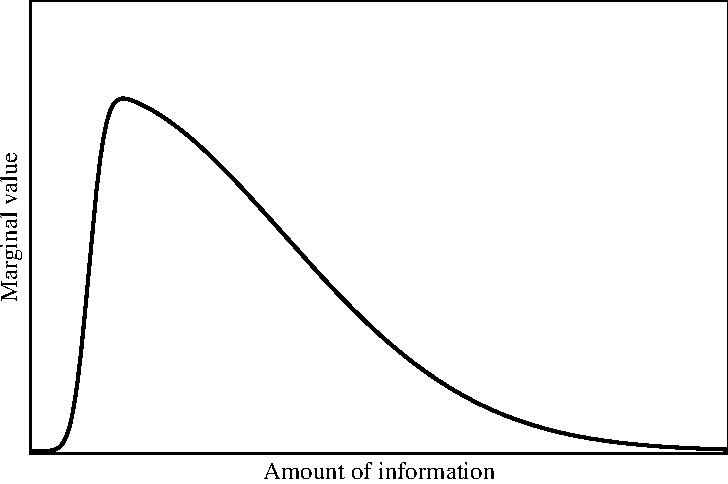
\includegraphics[width=0.8\textwidth]{figures/figradnerpres.pdf}
  \end{figure}

  \note{
    \begin{itemize}
      \item \cite{Radner1984} Nonconcavity (rising MB)
    \end{itemize}
  }
\end{frame}


\begin{frame}{problems with information}

  In general, information value doesn't have a nice, closed-form
  expression.


\end{frame}


%%%%%%%%%%%%%%%%%%%%%%%%%%%%%%%%%%%%%%%%%%%%%%%%%%%%%%%%%%%%%%%%%%%%%%%%
%% Results preview
%%%%%%%%%%%%%%%%%%%%%%%%%%%%%%%%%%%%%%%%%%%%%%%%%%%%%%%%%%%%%%%%%%%%%%%%

\section{Preview of results}
\label{sec:question}


\begin{frame}{what i do}

  To answer these questions I develop an \textbf{approximate} consumer theory for information.\\[1em]

  That is, I will
  \begin{itemize}
    \item<1-> Define a generalized notion of \textbf{precision}
          \begin{itemize}
            \item Demand approximately follows a maximin rule
          \end{itemize}
    \item<2-> Explore implications for consumer theory
  \end{itemize}\bigskip

  \onslide<3>{\alert{Information is \textbf{not} described by the convex-preference benchmark.}}

  \note{
    \begin{itemize}
      \item For illustration, will focus on classical constrained
            optimization problem
      \item Obviously MRS is useful in other settings.
      \item In a cardinal (quasi-linear setting) -> two-stage optimization
    \end{itemize}
  }
\end{frame}

\begin{frame}{what i do}
  \begin{figure}[h]
    \centering
   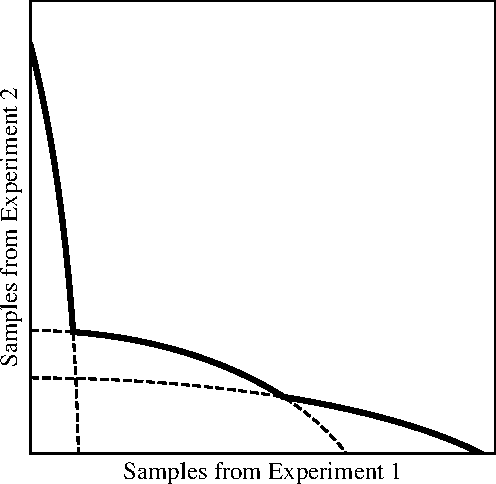
\includegraphics[width=0.7\textwidth]{figures/figqualitativepres.pdf}
  \end{figure}
  \note{%

  }
\end{frame}


\begin{frame}{what i do}

  \begin{itemize}
    \item<1-> This approximation will \textbf{not} depend on decision-maker
          characteristics (prior, utility function).\bigskip
    \item<2-> \ul{Everyone facing the same costs will agree on the optimal
          bundle at large samples.}
  \end{itemize}

  \note{
  }
\end{frame}

\begin{frame}{agenda}
  \tableofcontents
\end{frame}


%%%%%%%%%%%%%%%%%%%%%%%%%%%%%%%%%%%%%%%%%%%%%%%%%%%%%%%%%%%%%%%%%%%%%%%%
%% Literature
%%%%%%%%%%%%%%%%%%%%%%%%%%%%%%%%%%%%%%%%%%%%%%%%%%%%%%%%%%%%%%%%%%%%%%%%

\section{Literature}
\label{sec:literature}

\begin{frame}{agenda}
  \tableofcontents[currentsection]
\end{frame}


\begin{frame}{literature}

  Statistics:\\[1em]
  \cite{Chernoff1952} (Asymptotic relative efficiency)
  \begin{itemize}
    \item How many samples from one test needed to do as well as $n$ from another
    \item Comparison of extremes: all one or the other
    \item Only covers simple hypothesis tests (2 states)
  \end{itemize}\vspace{\baselineskip}\pause

  Contribution:
  \begin{itemize}
    \item<2->  Extend to local comparisons (MRS), and
    \item<2-> to arbitrary finite-action/finite-state problems.
  \end{itemize}

  \note{
    \begin{itemize}
      \item Trade offs between statistical tests
      \item Mixing tests usually doesn't make much sense because it's the same data
      \item Chernoff did recognize the application to experiment design but didn't consider the possibility of interior solutions.
      \item Can consider my result a local version of Chernoff's
    \end{itemize}
  }


  \note{%

  }
\end{frame}


\begin{frame}{literature}

  Economics:\\[1em]
  \cite{Moscarini2002}
  \begin{itemize}
    \item Apply similar methods to approximate info value and demand for information in the single source case
  \end{itemize}\vspace{\baselineskip}
  Contribution:
  \begin{itemize}
    \item<2-> Economic: extend this to environment with multiple sources.
    \item<2-> \footnotesize Technical: tighten the bounds on the convergence rate.
  \end{itemize}

  \note{%

  }
\end{frame}


\begin{frame}{other related literature}
  \textbf{Value of and comparisons between information sources}:\\
  \cite{Borgers2013}, \cite{Athey2018}, \&c.\vspace{\baselineskip}

  \textbf{Rational inattention:}\\
  \cite{Sims2003}, \&c.\vspace{\baselineskip}

  \textbf{Optimal experiment design:}\\
  \cite{Elfving1952}, \cite{Chernoff1953}, \cite{Dette2007}, \&c.\\

  \note{%
    \begin{itemize}
      \item Borgers: when are two samples complements for all DM'
      \item Athey: comparisons under a specific class of decision problems
    \end{itemize}
  }
\end{frame}


%%%%%%%%%%%%%%%%%%%%%%%%%%%%%%%%%%%%%%%%%%%%%%%%%%%%%%%%%%%%%%%%%%%%%%%%
%% Model
%%%%%%%%%%%%%%%%%%%%%%%%%%%%%%%%%%%%%%%%%%%%%%%%%%%%%%%%%%%%%%%%%%%%%%%%

\section{Model}
\label{sec:model}


\begin{frame}{agenda}
  \tableofcontents[currentsection,sectionstyle=show/shaded]
  \note{%

  }
\end{frame}


\begin{frame}{model -- environment}

  \begin{itemize}
    \item \alert<1>{Finitely many possible states of the world, $\theta \in \Theta$}
          \begin{itemize}
            \item DM prior, $\mathbf{p}\in\Delta\Theta$ (no degenerate beliefs)
          \end{itemize}
    \item<2-> \alert<2>{Finitely many possible actions, $a\in A$ }
    \item<3-> \alert<3>{DM state-dependent utility, $u(a,\theta)$}
          \begin{itemize}
            \item<3-> Assume each state has a unique and distinct optimal action
          \end{itemize}
    \item<4-> \alert<4>{DM chooses action to maximize expected payoff}\\[2em]
    \item<5-> \alert<5>{Prior to acting, DM can purchase information about the state.}
  \end{itemize}

  \note{%

  }
\end{frame}


\begin{frame}{model -- information sources}

  Information sources $\mathcal{E}_{1}, \mathcal{E}_{2}$\\
  AKA:\ tests, signals, (Blackwell) experiments

  \begin{itemize}
    \item<1-> \alert<1>{$\mathcal{E}_j\equiv \langle F_j(x \| \theta) \rangle$ ($x\in X$ realizations)}
    \item<2-> \alert<2->{Assume: ``thin tails''}
          \begin{itemize}
            \item<3-> $\Rightarrow$ no realization perfectly reveals or rules out any state.
          \end{itemize}
  \end{itemize}

  \note{%
    Can assume realizations are reals and that $F$ has a density
  }
\end{frame}


\begin{frame}[label=info-sources]{model - information sources}

  \begin{itemize}
    \item DM can purchase an arbitrary number of
          \textit{conditionally independent} samples, $n_i$, from each source at cost $\varepsilon c_i$ per sample
          \begin{itemize}
            \item $\varepsilon$ small\bigskip
          \end{itemize}
    \item For exposition, assume sources are \textbf{infinitely-divisible}, so fractional ``samples'' are allowed.\bigskip\pause
    \item DM has budget $Y$ to spend on info.\bigskip\pause

    \item \alert{After choosing a bundle of information $(n_1, n_2)$, DM observes the vector of realizations, and updates via Bayes Rule.}
  \end{itemize}

  \note{%

  }
\end{frame}


\begin{frame}{infinite-divisibility}

  \begin{definition}
    Say an information source, $\mathcal{E}$ is \textbf{infinitely-divisible} if for any $k$ there exists an information source $\mathcal{E}^{1/k}$ such that $k$ samples conditionally i.i.d. from $\mathcal{E}^{1/k}$ is equivalent to $1$ sample from $\mathcal{E}$.
  \end{definition}

  \note{%

  }
\end{frame}


\begin{frame}{infinite-divisibility}

  1/2 ``samples'' from $\E$ means 1 sample from $\E^{1/2}$
  \centering
  \begin{tikzpicture}%
    [>=stealth,
    shorten >=1pt,
    node distance=2cm,
    on grid,
    auto,
    every state/.style={draw=black!60, fill=black!5, very thick}
    ]
    \node[state] (mid)                  {$\mathcal{E}^{1/2}$};
    \node[state] (upper) [above=of mid] {$\mathcal{E}^{1/2}$};
    \node[state] (right) [right=of mid] {\Huge$\mathcal{E}$};

    \path[->]
    % FROM       BEND/LOOP           POSITION OF LABEL   LABEL   TO
    (upper) edge[bend left]     node                      {} (right)
    (mid)   edge[bend left=10]  node                      {} (right)
    ;
  \end{tikzpicture}

  \note{%

  }
\end{frame}



\begin{frame}{infinite divisibility - example}

  An infinitely-divisible analog of any experiment can be acheived by \textbf{Poissonizing} it.\bigskip

  Instead of choosing samples directly, DM chooses \textbf{expected samples} and then receives an appropriate Poisson draw of samples.\pause\bigskip

  Sum of Poissons is Poisson:\\
  \begin{center}
    1 sample from the Poissonization with 1 expected sample\\
    $\Leftrightarrow$\\
    2 samples from the Poissonization with 0.5 expected samples.
  \end{center}
  \note{%

  }
\end{frame}



\begin{frame}{model -- expected loss}

  Expected difference in value of acting correctly and acting with information
  \begin{align*}
    L(&n_1, n_2) = \\
      & \sum_{\theta}p_{\theta}
        \left[ \int_{x} \underbrace{
        \left( u(a^{*}(\theta), \theta) - u(a(\mathbf{x}), \theta) \right)
        }
        f_{n_1, n_2}(x\|\theta)\D x
        \right]
  \end{align*}
  \hspace{4em}{\small cost of choosing $a(x)$ when $a(\theta)$ optimal}\\[2em]\pause

  \alert{Goal: Minimize subject to budget constraint}\\
  {\small\hspace{1em}(equivalent to maximizing value of information)}
  \note{%
    Averaging over all possible mistakes
  }
\end{frame}


\begin{frame}{model -- expected loss}

  \begin{figure}[h]
    \centering
    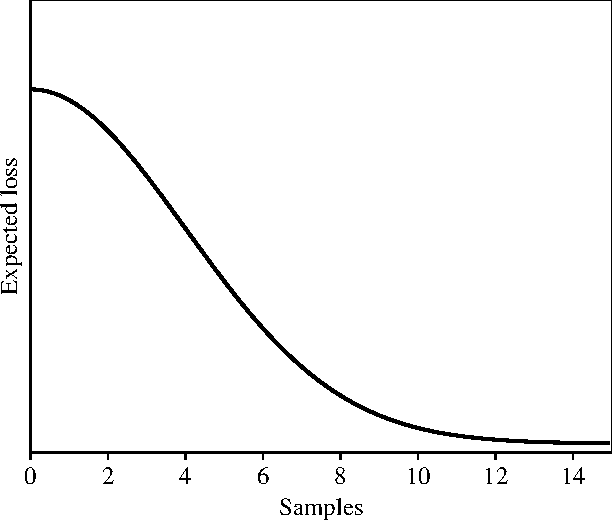
\includegraphics[width=0.8\textwidth]{figures/figlosspres.pdf}
  \end{figure}

  \note{%

  }
\end{frame}


\begin{frame}{approach}


  \begin{enumerate}
    \item<1-> Review the relevant large-deviations approximations
          \begin{itemize}
            \item Generalize to the multi-source model
          \end{itemize}
    \item<2-> Transform into a ``utility function''
          \begin{itemize}
            \item Define \textbf{precision}
          \end{itemize}

    \item<3-> Examine properties of the approximation and implications for demand
  \end{enumerate}

  \note{%

  }
\end{frame}


%%%%%%%%%%%%%%%%%%%%%%%%%%%%%%%%%%%%%%%%%%%%%%%%%%%%%%%%%%%%%%%%%%%%%%%%
%% Large-deviations approximations
%%%%%%%%%%%%%%%%%%%%%%%%%%%%%%%%%%%%%%%%%%%%%%%%%%%%%%%%%%%%%%%%%%%%%%%%

\section{Large-deviations approximations}
\label{sec:large-deviations}


%%%%%%%%%%%%%%%%%%%%%%%%%%%%%%%%%%%%%%%%%%%%%%%%%%%%%%%%%%%%%%%%%%%%%%%%
%% Two states
%%%%%%%%%%%%%%%%%%%%%%%%%%%%%%%%%%%%%%%%%%%%%%%%%%%%%%%%%%%%%%%%%%%%%%%%

\subsection{Two states}
\label{sec:two-states}

\begin{frame}{agenda}

  \tableofcontents[currentsection,sectionstyle=show/shaded]

  \note{
    The two state case will serve as a building block for the general case.
  }
\end{frame}


\begin{frame}{two states -- setup}

  \begin{itemize}
    \item States:
          \begin{itemize}
            \item Null hypothesis -- $H_0$
            \item Alternative hypothesis -- $H_1$
            \item Prior that alternative is true -- $p$\bigskip
          \end{itemize}

    \item<2-> Actions
          \begin{itemize}
            \item<2-> Accept the null -- $\mathcal{A}$
            \item<2-> Reject the null -- $\mathcal{R}$
          \end{itemize}
  \end{itemize}

  \note{%

  }
\end{frame}


\begin{frame}{two states -- expected loss}

  \begin{align*}
    L(n_1,n_2) = &\alert<1>{(1-p)\alert<3>{\alpha_{I}(n_1,n_2)}
                   \overbrace{\big(
                   u(\mathcal{A}, H_0) - u(\mathcal{R}, H_0)
                   \big)}^{\text{loss from Type-I error}}}\\
                 &\hspace*{0.9em}+ \alert<2>{p\,\alert<3>{\alpha_{II}(n_1,n_2)}
                   \underbrace{\big(
                   u(\mathcal{R}, H_1) - u(\mathcal{A}, H_1)
                   \big)}_{\text{loss from Type-II error}}}
  \end{align*}

  \begin{itemize}
    \item \alert<3>{$\alpha_{I}$} -- Probability of Type-I error
    \item \alert<3>{$\alpha_{II}$} -- Probability of Type-II error\bigskip
  \end{itemize}

  \onslide<3->{\centering\alert{\textsc{goal:}} Approximate error probabilities}

  \note{%

  }
\end{frame}


\begin{frame}{error probabilities}

  Start with the one-source case

  \begin{multline*}
    \alpha_I(n) = \\
    \mathbb{P} \left(
      {p \prod_{k=1}^n f(x_{k}\|H_1)
        \over
        p \Pi_{k=1}^n f(x_k\| H_1) + (1-p) \Pi_{k=1}^n f(x_k\| H_0)}
      > \bar{p}
      \ \bigg|\  H_{0}
    \right)
  \end{multline*}

  \note{%

  }
\end{frame}


\begin{frame}{error probabilities}

  Change to log-likelihood ratios:

  \begin{align*}
    &\alpha_I(n)\\
    &\hspace{-1.1em}= \mbox{\normalsize $\mathbb{P}\left(
      \log \left( p \over 1-p \right)
      + \sum_{k=1}^n \alert<2>{\log \left( f(x_k\|H_1) \over f(x_k\|H_0) \right)}
      >
      \log \left( \bar{p} \over 1-\bar{p}\right)\ \bigg|\ H_0
      \right)$}\\[1em]
    \onslide<2->{
    &\hspace{-1.1em}=
      \mathbb{P}\left(
      \sum_{k=1}^n \alert<2>{s_k} > \bar{l} - l \bigg|\ H_{0}
      \right)
      }
  \end{align*}\pause

  \note{%

  }
\end{frame}

\begin{frame}{error probabilities}

  \begin{equation*}
    \alpha_I(n)  =
    \mathbb{P}\left(
      \sum_{k=1}^n s_k > \bar{l} - l
    \right)
  \end{equation*}

  If we divide by $n$, we have a statement about sample averages.\\[1em]\pause
  But can't use CLT:\, $\mathbb{E}(s_{i})<0$ errors happen far from the mean.\\

  This is a \textbf{large} deviation.\hfill \link{large-dev}{more info}

  \note{%

  }
\end{frame}


\begin{frame}[label=approximation]{efficiency index}

  Large deviations approximations often depend on a minimized moment generating function:
  \begin{align*}
    \rho &\equiv \min_t M(t)\\
         &= \min_t \int e^{t\log \left( f(x\|H_1) \over f(x\|H_0) \right)} f(x\|H_0)\D x\\
         &= \alert{\min_t \int {f(x\|H_1)}^{t} {f(x\|H_0)}^{1-t}\D x}
  \end{align*}


  \note{%

  }
\end{frame}

\begin{frame}{efficiency index}


  \begin{equation*}
    \rho=\min_t \int {f(x\|H_1)}^{t} {f(x\|H_0)}^{1-t}\D x
  \end{equation*}
  Call $\rho$ the (Chernoff) \textbf{efficiency index} of the information source.\\
  Properties:
  \begin{itemize}
    \item<1-> \alert<1>{$\rho\in(0,1)$}
    \item<2-> \alert<2>{Blackwell more informative $\Rightarrow$ \textbf{lower} index}
    \item<3-> \alert<3>{$n$ i.i.d. samples has index $\rho^n$}
    \item<4-> \alert<4>{Doesn't depend on DM characteristics}
  \end{itemize}

  \note{%

  }
\end{frame}


\begin{frame}{large-deviation approximation}

  Large-deviations probabilities fall \textbf{exponentially}: error probabilities are roughly proportional to
  \begin{equation*}
    \alert{\frac{\rho^n}{\sqrt{n}}
    }  \end{equation*}
  \only<2>{
    \begin{lemma}[MS02]
      The expected loss from $n$ samples from an information source with efficiency index $\rho$ is
      \begin{equation*}
        L(n) \propto \frac{\rho^{n}}{\sqrt{n}}
        \left(1 + O\left(1 \over \sqrt{n}\right)\right)
      \end{equation*}
    \end{lemma}
  }
  \onslide<3>{
    \begin{lemma}[MS02*]
      The expected loss from $n$ samples from an information source with efficiency index $\rho$ is
      \begin{equation*}
        L(n) \propto \frac{\rho^{n}}{\sqrt{n}}
        \left(1 + O\left(1 \over n\right)\right)
      \end{equation*}
    \end{lemma}
  }
  \note{%

  }
\end{frame}


\begin{frame}{to multiple sources}

  \begin{tabular}{rr}
    $N=n_1+n_2$: & \textbf{total sample size}\\
    $r=n_1/N$: & \textbf{composite factor}\bigskip\pause
  \end{tabular}

  MGF of a sum is the product of MGFs
  \begin{align*}
    {M_1(t)}^{n_1}{M_2(t)}^{n_2} = \left(
    \alert{{M_1(t)}^{r}{M_2(t)}^{1-r}}
    \right)^N
    \equiv \alert{M_r(t)}^{N}
  \end{align*}\pause
  Define the \textbf{$r$-composite} efficiency index
  \begin{equation*}
    \rho_r \equiv \min_t {M_r(t)}
  \end{equation*}\pause
  and similarly the \textbf{$r$-marginal} efficiency indices
  \begin{equation*}
    \rho_{ri} = M_i(\tau_r)
  \end{equation*}

  so $\rho_r=\rho_{r1}^r\rho_{r2}^{1-r}$

  \note{%

  }
\end{frame}


\begin{frame}{loss with multiple sources}

  Plugging things in, we have
  \begin{align*}
    L(n_1,n_2) &= A(r){\rho_r^N\over \sqrt{N}}
                 \left( 1 + O \left( 1 \over N \right) \right)\\[1em]
               &= \alert{A(r){\rho_{r1}^{n_1}\rho_{r2}^{n2} \over \sqrt{n_1+n_2}}
                 \left( 1 + O \left( 1 \over n_1 + n_2 \right) \right)}
  \end{align*}
  where $A$ depends only on the relative sample proportions $r$.

  \note{%

  }
\end{frame}


\begin{frame}{foreshadowing}

  The marginal index is the MGF evaluated at the minimizer for the composite.

  So we have:
  \begin{equation*}
    \rho_r = \rho_{r1}^r\rho_{r2}^{1-r} \alert{\geq} \rho_1^r\rho_2^{1-r}
  \end{equation*}\pause

  Composite experiments perform \textbf{worse} than the sum of their parts.

  \hfill\link{2state-intuition}{intuition}
  \note{%

  }
\end{frame}

\begin{frame}[label=2state-summary]{to review}
  \begin{itemize}
    \item Defined the \textbf{efficiency index}, $\rho$\bigskip
    \item Losses fall exponentially fast in $\rho$ with sample\bigskip
    \item Introduced the \textbf{marginal} efficiency index, $\rho_{rj}$
          \begin{itemize}
            \item loss is reduced by roughly a factor of $\rho_{r1}$ consuming a sample from $\E_1$ in addition to a bundle with sample proportions $r$
          \end{itemize}
  \end{itemize}
  \note{%

  }
\end{frame}

%%%%%%%%%%%%%%%%%%%%%%%%%%%%%%%%%%%%%%%%%%%%%%%%%%%%%%%%%%%%%%%%%%%%%%%%
%% Many states
%%%%%%%%%%%%%%%%%%%%%%%%%%%%%%%%%%%%%%%%%%%%%%%%%%%%%%%%%%%%%%%%%%%%%%%%


\subsection{Many states}
\label{sec:many-states}

\begin{frame}{agenda}

  \tableofcontents[currentsubsection,sectionstyle=show/shaded]

  \note{
    The two state case will serve as a building block for the general case.
  }
\end{frame}



\begin{frame}{generalizing to multiple states}

  \begin{itemize}
    \item<1-> With multiple states, we now have many log-likelihood ratio
          distributions:
          \begin{itemize}
            \item<2-> e.g. With three states, we have $\theta_1$ vs $\theta_2$, $\theta_1$ vs $\theta_3$, and $\theta_2$ vs $\theta_3$
                  LLRs.
          \end{itemize}
    \item<3-> So for $\E_i$ we can define an efficiency index for each pair
          of states
          \onslide<3->{
          \begin{equation*}
            \rho_{i}(\theta,\theta') \equiv
            \min_t \int f(r\|\theta)^t f(r\|\theta')^{1-t} \D r
          \end{equation*}}
  \end{itemize}

  \note{%

  }
\end{frame}


\begin{frame}{expected loss}
  \begin{multline*}
    L(n_1,n_2) \\
    = \sum_\theta p_\theta \sum_{\theta'\neq \theta}
    \overbrace{
      \alpha(n_1,n_2\,;\,a,\theta)}^{\text{mistake prob.}}
    \underbrace{
      (u(a^{*}(\theta),\theta) - u(a, \theta))}_{
      \text{Loss from choosing a}}
  \end{multline*}


  \note{%

  }
\end{frame}


\begin{frame}{expected loss approximation}

  Intuition:

  \begin{itemize}
    \item<1-> Expected loss is a sum of mistake probabilities
    \item<2-> Mistake probabilities fall \textbf{exponentially}
    \item<3-> \alert<3>{Sum of exponentials $\Rightarrow$ \textbf{biggest} term eventually dominates}
  \end{itemize}



  \note{%

  }
\end{frame}


\begin{frame}{expected loss approximation}

  Applying a lemma of MS02, we have
  \begin{align*}
    &L(n_1,n_2) = A(r){\textstyle \max_{\theta,\theta'}\left\{ \rho_r(\theta,\theta')^N \right\}
      \over \sqrt{N}}
      \left( 1 + O \left( 1 \over N \right) \right)\\[1em]
    &= \alert{
      A(r){\textstyle \max_{\theta,\theta'}\left\{ \rho_{r1}(\theta,\theta')^{n_1}\rho_{r2}(\theta,\theta')^{n_2} \right\}
      \over \sqrt{n_1+n_2}}
      \left( 1 + O \left( 1 \over N\right) \right)}
  \end{align*}
  where $A$ depends only the relative sample proportions.

  \note{%

  }
\end{frame}


\begin{frame}{to review}

  \begin{itemize}
    \item Efficiency index for each pair of states
          \begin{itemize}
            \item How well does an experiment distinguish between a pair of states
          \end{itemize}\bigskip
    \item<2-> Loss dominated by most likely mistake, i.e. \textbf{highest} index
  \end{itemize}
  \note{%

  }
\end{frame}


\begin{frame}{approach}

  \begin{enumerate}
    \item Review the relevant large-deviations approximations \alert{\CheckedBox}
          \begin{itemize}
            \item Generalize to the multi-source model \alert{\CheckedBox}
          \end{itemize}
    \item \alert{Transform into a ``utility function''}
          \begin{itemize}
            \item Define \textbf{precision}
          \end{itemize}
    \item Examine properties of the approximation and implications for demand
  \end{enumerate}

  \note{%

  }
\end{frame}

\begin{frame}{precision}

  The multiplicative form of the approximation screams to have logs taken:\bigskip

  In the one-source, two-state world:
  \begin{equation*}
    -\log(L(n)) = n \alert{\beta}
    \left( 1 + O \left( \log(n)  n^{-1} \right) \right)
  \end{equation*}

  Call \alert{$\beta\equiv -\log(\rho)$} the \textbf{precision} of the experiment\pause\bigskip

  Properties

  \begin{itemize}
    \item \alert<2>{$\beta>0$}
    \item<3-> \alert<3>{Blackwell more informative \Rightarrow \textbf{higher} precision}
    \item<4-> \alert<4>{$n$ i.i.d. samples has precision $n\beta$}
  \end{itemize}

  \note{%

  }
\end{frame}


\begin{frame}{precision -- example}

  \begin{tabbing}
    Gaussian noise: \= $r\sim \mathcal{N}(0,\sigma^2)$ in state $H_0$\\
    \> $r\sim \mathcal{N}(\mu,\sigma^2)$ in state $H_1$
  \end{tabbing}

  \begin{itemize}
    \item<2-> Precision is $\beta =
          \frac{1}{8}\frac{\mu^2}{\sigma^2}$
          \begin{itemize}
            \item<3-> Proportional to the signal-to-noise ratio
            \item<3-> Proportional to the classical notion of precision ($1/\sigma^2$)
          \end{itemize}
  \end{itemize}

  \note{%

  }
\end{frame}


\begin{frame}{marginal precision}

  Similarly, define the \textbf{$r$-composite} precision and \textbf{$r$-marginal} precisions.

  \begin{align*}
    -\log(\rho_r)
    \equiv \alert{\beta_r} & \alert{=r\beta_{r1} + (1-r)\beta_{r2}}\\
                  &\equiv -r\log(\rho_{r1}) - (1-r)\log(\rho_{r2})
  \end{align*}

  \note{%

  }
\end{frame}


\begin{frame}{precision and utility}

  Putting it all together we have
  \begin{align*}
    -&\log(L(n_1,n_2)) = \min_{\theta,\theta'} \left\{ N\beta_r(\theta,\theta') \right\}
       \left(
       1 + O \left( \log(N) \over N \right)
       \right)\\[1em]
     &= \alert{\min_{\theta,\theta'}
       \left\{ n_1\beta_{r1}(\theta,\theta') + n_2\beta_{r2}(\theta,\theta') \right\}}
       \left(
       1 + O \left( \log(N) \over N \right)
       \right)
  \end{align*}\pause

  at high enough total samples, prefer bundles with higher total \textbf{minimum} (worst-case) precision!

  \note{%

  }
\end{frame}


\begin{frame}{to review}


  \begin{itemize}
    \item Defined a generalized notion of \textbf{precision} and \textbf{marginal} precision
          \begin{itemize}
            \item Approximate utility and marginal utility for information
          \end{itemize}\bigskip
    \item<2-> \textbf{Remember:} Precision independent of DM characteristics
          \begin{itemize}
            \item<2-> Everyone agrees on ranking of bundles at large samples
          \end{itemize}
  \end{itemize}

  \note{%

  }
\end{frame}

\begin{frame}{approach}

  \begin{enumerate}
    \item Review the relevant large-deviations approximations \alert{\CheckedBox}
          \begin{itemize}
            \item Generalize to the multi-source model \alert{\CheckedBox}
          \end{itemize}
    \item Transform into a ``utility function'' \alert{\CheckedBox}
          \begin{itemize}
            \item Define \textbf{precision} \alert{\CheckedBox}
          \end{itemize}
    \item \alert{Examine properties of the approximation and implications for demand }
  \end{enumerate}

  \note{%

  }
\end{frame}


%%%%%%%%%%%%%%%%%%%%%%%%%%%%%%%%%%%%%%%%%%%%%%%%%%%%%%%%%%%%%%%%%%%%%%%%
%% Consumer theory
%%%%%%%%%%%%%%%%%%%%%%%%%%%%%%%%%%%%%%%%%%%%%%%%%%%%%%%%%%%%%%%%%%%%%%%%

\section{Consumer theory}
\label{sec:consumer-theory}


\begin{frame}{agenda}

  \tableofcontents[currentsection,sectionstyle=show/shaded]

  \note{%

  }
\end{frame}




%%%%%%%%%%%%%%%%%%%%%%%%%%%%%%%%%%%%%%%%%%%%%%%%%%%%%%%%%%%%%%%%%%%%%%%%
%% Demand for samples
%%%%%%%%%%%%%%%%%%%%%%%%%%%%%%%%%%%%%%%%%%%%%%%%%%%%%%%%%%%%%%%%%%%%%%%%

\subsection{Demand for samples}
\label{sec:demand}


\begin{frame}{demand for cheap information}

  \begin{proposition}[Maximin precision]
    For budget $Y$ and per sample costs $\varepsilon c_1$ and $\varepsilon c_2$ optimal sample demand is
    \begin{multline*}
      (n_1^{*},n_2^{*}) \\
      =
      \mbox{\normalsize$\left(
          \argmax_{n_1,n_2} \min_{\theta,\theta'}
          \left\{ n_1 \beta_{r1}(\theta,\theta') + n_2 \beta_{r2}(\theta,\theta') \right\}
        \right)$}\\
      \mbox{\normalsize $\times\left(
          1 + O \left( \varepsilon \right)
        \right)$}
    \end{multline*}
    subject to $\varepsilon(n_1c_1+n_2c_2)\leq Y$.
  \end{proposition}\pause\bigskip

  Can treat total worst-case precision \textbf{as if} utility.

  \note{%

  }
\end{frame}


\begin{frame}{precision per dollar}

  Since precision is homothetic, we can equivalently say the optimal sample proportions maximize \textbf{precision per dollar}
  \begin{align*}
    r^{*} = \argmax_r \left\{ \min_{\theta,\theta'} \left\{
    \frac{\beta_r(\theta,\theta')}{rc_1+(1-r)c_2}
    \right\} \right\}
  \end{align*}

  \note{%

  }
\end{frame}


\begin{frame}{corners?}

  Recall composites are worse than the sum of their parts for a fixed dichotomy:
  \begin{equation*}
    \rho_{r1}^{n_1}\rho_{r2}^{n_2} \alert{\geq} \rho_1^{n_1}\rho_2^{n_2}
    \hspace{1em} \Leftrightarrow \hspace{1em}
    n_1\beta_{r1} + n_2\beta_{r2} \alert{\leq} n_1\beta_{1} + n_2\beta_{2}
  \end{equation*}\bigskip

  Corners always optimal?

  \note{%

  }

\end{frame}


\begin{frame}{iso-least-precision curves}

  \begin{center}
    \begin{tikzpicture}[scale=0.8]
      % axes
      \draw [->] (0,0) -- (5.5,0) node [below] {$n_1$};
      \draw [->] (0,0) -- (0,5.5) node [left] {$n_2$};

      % ICs
      \draw [dashed] (0,4) .. controls (1,3.4) and (2.6,1) .. (3,0);
      \onslide<1>{\draw [-,line width=1.5pt] (0,4) .. controls (1,3.4) and (2.6,1) .. (3,0);}

      \onslide<2->{\draw (1,3.5) node [right] {1,2 dichotomy is worst};}
      \onslide<2->{\draw [dashed] (0,3) .. controls (1,2.6) and (3.4,1) .. (4,0);}
      \onslide<2->{\draw (3.5,1) node [right] {1,3 dichotomy is worst};}
      \onslide<2->{\draw [dashed] (0,2) .. controls (0.6,1.6) and (1.65,0.6) .. (2,0);}

      % Draw outer contour
      \onslide<3->{
        \draw [-,line width=1.5pt]
        (0,4) .. controls (1,3.4) and (1.885,1.885) .. (1.885,1.885);
        \draw [-,line width=1.5pt]
        (1.885,1.885) .. controls (1.885,1.885) and (3.4,1) .. (4,0);
      }
    \end{tikzpicture}
  \end{center}
  \only<1,2>{For a single dichotomy, iso-precision curves \textbf{bow out}}
  \only<3->{But the outer contour has inward pointing kinks}
  \note{%

  }
\end{frame}


\begin{frame}{properties of precision}

  \begin{lemma}
    For a fixed dichotomy, total precision is homothetic and (quasi)convex.\\
    Worst-case precision is thus homothetic and \alert{locally} quasiconvex at almost all sample proportions $r$.
  \end{lemma}

  \hfill\link{local-convex}{more info}
  \note{%

  }
\end{frame}


\begin{frame}{income elasticity}

  Information sources are always normal goods at large samples.\bigskip

  \begin{corollary}[Income elasticity]
    The (arc) income elasticity of demand given a fixed change in budget is $1+O(\varepsilon)$.
  \end{corollary}

  \note{%

  }
\end{frame}


\begin{frame}[label=maximin-prec]{demand at kinks}

  \begin{proposition}[corners or kinks]
    The set of sample proportions that maximize worst-case precision for some cost vector and budget is finite.
    \begin{equation*}
      \mbox{\footnotesize $\left|\left\{ r^{*} : \exists c_1,c_2,Y \text{ s.t. }
            r^{*}\in \argmax_{r} \{\min_{\theta,\theta'}\beta_r(\theta,\theta')/(rc_1+(1-r)c_2)\}
          \right\}\right|
        < \infty$ }
    \end{equation*}
  \end{proposition}

  \note{%

  }
\end{frame}


\begin{frame}{locally perfect complements}

  Info behaves (locally) like \textbf{perfect complements}:

  \begin{corollary}[Price elasticity]
    At almost all costs, the (arc) price elasticity of demand for samples from all sources given a small percent change, $\delta$, of $c_1$ is
    \begin{align*}
      \eta_1 =& { rc_1 \over rc_1 + (1-r)c_2 }\left( 1 + O \left( \varepsilon + \delta \right) \right)
    \end{align*}
  \end{corollary}\pause

  But the sample bundle changes drastically around costs that jump between kinks!

  \note{%

  }
\end{frame}


\begin{frame}{bundle complexity}

  In a two-state environment (one dichotomy) only corners were possible.\bigskip

  Hints that ``sophisticated'' sample demand requires complicated environments.\bigskip\pause

  \begin{proposition}
    The maximin precision sample bundle has support on at most distinct information sources as there are dichotomies---i.e. $|\Theta|(|\Theta-1|)/2$.
  \end{proposition}

  \note{%

  }
\end{frame}


%%%%%%%%%%%%%%%%%%%%%%%%%%%%%%%%%%%%%%%%%%%%%%%%%%%%%%%%%%%%%%%%%%%%%%%%
%% Substitutability
%%%%%%%%%%%%%%%%%%%%%%%%%%%%%%%%%%%%%%%%%%%%%%%%%%%%%%%%%%%%%%%%%%%%%%%%

\subsection{Substitutability of samples}
\label{sec:label}

\begin{frame}{agenda}

  \tableofcontents[currentsubsection,sectionstyle=show/shaded]

  \note{
  }
\end{frame}


\begin{frame}{marginal rate of substitution}

  Solutions are at kinks so there isn't much use for MRS in a classic budget-constrained environment.\bigskip\pause

  But information is weird:

  \begin{itemize}
    \item<2-> Often non-rival, non-excludable
    \item<3-> Often have additional constraints (finite-sample datasets)
  \end{itemize}\pause\bigskip

  Might want to understand what happens away from the kinks.

  \note{%

  }
\end{frame}


\begin{frame}{marginal rate of substitution}

  \begin{proposition}
    If the worst-case dichotomy, $D$, is unique at sample proportion $r$, then the marginal rate of substitution is
    \begin{equation*}
      \frac{\partial L / \partial n_1}{\partial L / \partial n_2}
      = \frac{\beta_{r1}(D)}{\beta_{r2}(D)}
      \left( 1 + O\left( {1 \over n_1 + n_2} \right) \right)
    \end{equation*}
  \end{proposition}\bigskip\pause

  Samples are substitutable in proportion to their marginal precisions.\bigskip

  \hfill\link{discrete-mrs}{discrete version}
  \note{%

  }
\end{frame}


%%%%%%%%%%%%%%%%%%%%%%%%%%%%%%%%%%%%%%%%%%%%%%%%%%%%%%%%%%%%%%%%%%%%%%%%
%% Numerical results
%%%%%%%%%%%%%%%%%%%%%%%%%%%%%%%%%%%%%%%%%%%%%%%%%%%%%%%%%%%%%%%%%%%%%%%%

\section{How good is the approximation?}
\label{sec:simulations}

\begin{frame}[label=sims]{agenda}

  \tableofcontents[currentsubsection,sectionstyle=show/shaded]

  \note{
  }
\end{frame}

\begin{frame}{sources of error}

  Two sources of approximation error:

  \begin{enumerate}
    \item<1-> \alert<1>{Large-deviations approximation for single mistake probability}
    \item<2-> \alert<2>{Throwing out all but the most likely mistake}
  \end{enumerate}

  \note{%

  }
\end{frame}


\begin{frame}{sources of error}

  Large-deviations errors are small by the standards of large-sample approximations (CLT is $O(n^{-1/2})$)\bigskip\pause

  Ignoring less likely mistakes is fine so long as next most likely mistake isn't particularly close\bigskip\pause

  Approximation works best when the total number of possible states is small.

  \note{%

  }
\end{frame}


\begin{frame}{sources of error}

  \begin{figure}[h]
    \centering
    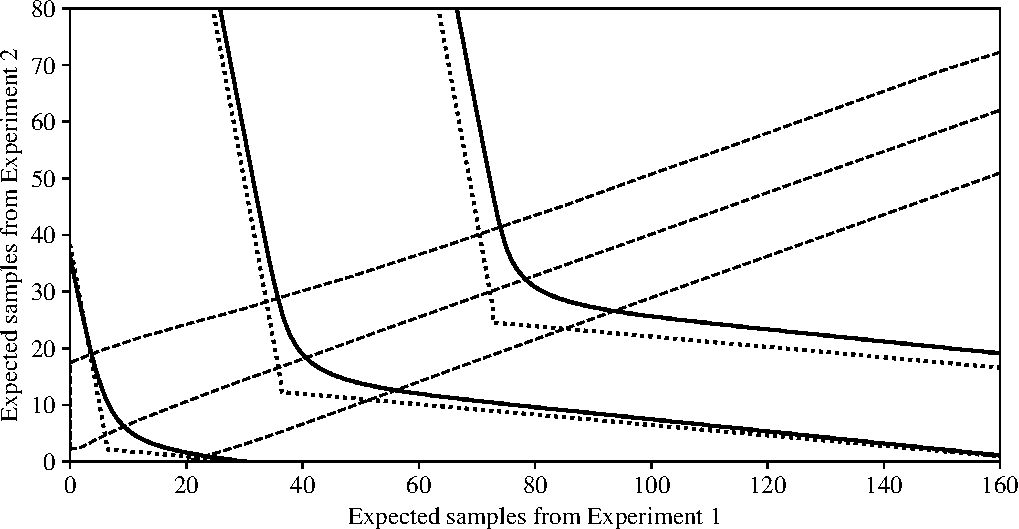
\includegraphics[width=\textwidth]{figures/poissonincexp.pdf}
  \end{figure}

  \note{%

  }
\end{frame}


%%%%%%%%%%%%%%%%%%%%%%%%%%%%%%%%%%%%%%%%%%%%%%%%%%%%%%%%%%%%%%%%%%%%%%%%
%% Conclusion
%%%%%%%%%%%%%%%%%%%%%%%%%%%%%%%%%%%%%%%%%%%%%%%%%%%%%%%%%%%%%%%%%%%%%%%%

\section{Conclusion and future work}
\label{sec:conclusion}

\begin{frame}{agenda}

  \tableofcontents[currentsubsection,sectionstyle=show/shaded]

  \note{
  }
\end{frame}


\begin{frame}{conclusion}


  \begin{itemize}
    \item Defined a general notion of \textbf{precision}
    \item Showed demand can be approximately analyzed treating precision \textbf{as if} it were a utility function
  \end{itemize}

  \note{%

  }
\end{frame}


\begin{frame}{conclusion}


\begin{itemize}
\item Information demand behaves as though indifference curves were locally bowed out, kinked, and homothetic
  \item Locally, sources are perfect complements
\end{itemize}
\begin{center}
    \begin{tikzpicture}[scale=0.5]
      % axes
      \draw [->] (0,0) -- (5.5,0) node [below] {$n_1$};
      \draw [->] (0,0) -- (0,5.5) node [left] {$n_2$};

      % ICs

      % Draw outer contour
      \onslide<1->{
        \draw [-,line width=1.5pt]
        (0,4) .. controls (1,3.4) and (1.885,1.885) .. (1.885,1.885);
        \draw [-,line width=1.5pt]
        (1.885,1.885) .. controls (1.885,1.885) and (3.4,1) .. (4,0);
      }
    \end{tikzpicture}
  \end{center}
  \note{%

  }
\end{frame}



\begin{frame}{implications}

  \begin{itemize}
    \item Suggests a form for information demand for applied work
          \begin{itemize}
            \item Treat information as a good with care\\
                  (preferences are \textbf{not} convex)\bigskip
          \end{itemize}
    \item<2-> Suggests a Bayesian approach to optimal experiment design
          \begin{itemize}
            \item Interior solutions matter
          \end{itemize}
  \end{itemize}

  \note{%

  }
\end{frame}


\begin{frame}{future work: infinite states}

  Most statistical problems are ones of \textbf{estimation}.\bigskip

  Unknown state is a real-valued parameter.\pause\bigskip

  \alert{\textsc{problem:}} As two states get close, the precision goes to zero.

  \hfill\link{infinite-state-approach}{na\"ive approach}
  \note{%

  }
\end{frame}


\begin{frame}[label=end]

  \centering
  \vspace{3em}
  {\Huge \alert{\textsc{thank you!}}}\\[2em]
  \textsc{\alert{email:}} gary.baker@wisc.edu\\
  \textsc{\alert{website:}} garygbaker.com
  \note{%

  }
\end{frame}


%%%%%%%%%%%%%%%%%%%%%%%%%%%%%%%%%%%%%%%%%%%%%%%%%%%%%%%%%%%%%%%%%%%%%%%%
%% Optional slides
%%%%%%%%%%%%%%%%%%%%%%%%%%%%%%%%%%%%%%%%%%%%%%%%%%%%%%%%%%%%%%%%%%%%%%%%


\begin{frame}[label=large-dev]{large vs small deviations}

  \begin{itemize}
    \item Could we just use a CLT?
          \begin{itemize}
            \item No: CLT approximates
                  $\mathbb{P}(\bar{x}_n-\mu < \epsilon/\sqrt{n})$
            \item Pr. that the deviation from the true mean is bigger than
                  some shrinking cutoff
            \item i.e. that the deviation is \underline{small}.
          \end{itemize}\vspace{\baselineskip}

    \item We have
          $\mathbb{P}(\bar{x}_n-\mu > -\mu + L/n)$
          \begin{itemize}
            \item Pr. that the deviation from the true mean is more than a
                  fixed amount
            \item This is a \textbf{large} deviation.
          \end{itemize}
  \end{itemize}
  \hfill\link{approximation}{\huge back}

  \note{%

  }
\end{frame}


\begin{frame}[label=2state-intuition]{intuition}
  The minimizer, $\tau$, is heuristically a measure of \textbf{slant}.

  Consider 2 news sources reporting about 2 candidates (R and
  L):
  \resizebox{\columnwidth}{!}{%
    \begin{tabular}[c]{|l|c|c||c|c|}
      \hline\normalsize
      & \multicolumn{2}{|c||}{Source 1 (R leaning)} &
                                                      \multicolumn{2}{|c|}{Source
                                                      2 (L leaning)}\\ \hline
      Truth $\backslash$ Report & favors R & favors L & favors R & favors L\\ \hline
      R actually better & 0.99     & 0.01     & 0.02     & 0.98 \\ \hline
      L actually better & 0.98     & 0.02     & 0.01     & 0.99\\ \hline
    \end{tabular}}

  Precision of both is the same, but minimizers are far
  apart.

  \onslide<2->{\small In this case, most decision makers will prefer 2
    samples from one or the other over 1 from each because 97\% of the
    time, the two sources will send contradictory signals.}

  \hfill\link{2state-summary}{back}
  \note{%
    DM with strong prior that L is true will favor Source 2 because
    information is only valuable if it can change her vote. The R
    recommendation from Source 2 moves the belief a lot.\\

    The L recommendation would also move her belief a lot, but in a
    direction she already favored. Her prior was already to vote for
    L.\\

    Could possibly think of this as a reason for polarization in media
    consumption.
  }
\end{frame}


\begin{frame}[label=local-convex]{local (quasi)convexity}

  \begin{definition}
    Say a function, $f$, is \alert{locally (quasi)convex} around a point $x$ if for $\varepsilon$ small enough $f$ is (quasi)convex on $B(x,\varepsilon)$.
  \end{definition}\bigskip

  \hfill\link{maximin-prec}{\huge back}
  \note{%

  }
\end{frame}


\begin{frame}[label=discrete-mrs]{discrete analog to mrs}

  \begin{proposition}
    Suppose $\mathcal{E}_1, \mathcal{E}_2$ not infinitely divisible. If there is a unique worst-case dichotomy at sample proportions, $r$, then the minimum number of samples from $\mathcal{E}_2$, $k_2$, required to minimally compensate for a loss of $k_1$ samples from $\mathcal{E}_1$ is exactly
    \begin{equation*}
      k_2 = \left\lceil k_{1} \frac{\beta_{r1}(D)}{\beta_{r2}(D)} \right\rceil
    \end{equation*}
    for $n_1+n_2$ high enough.
  \end{proposition}
  \hfill\link{sims}{\huge back}
  \note{%

  }
\end{frame}

\begin{frame}[label=infinite-state-approach]{infinite states: na\"{i}ve approach}

  Heuristically, the state hardest to distinguish from $\theta$ is the
  one ``adjacent'' to it, $\theta+d\theta$\vspace{\baselineskip}

  With some work, it happens to be the case that
  \begin{equation*}
    \beta(\theta,(\theta+d\theta)) = \underbrace{\int
      \frac{\D ^2}{\D \theta^2}\log(f(r|\theta))\D r}_{\hat{\beta}(\theta)} \, \D \theta^2
  \end{equation*}

  Roughly, $\hat{\beta}(\theta)$ measures how well a source can
  distinguish $\theta$ from nearby states.

  \onslide<2->{But you might know $\hat{\beta}(\theta)$ by another
    name: \ul{Fisher information}}

  \note{%
    $\hat{\beta}$ then is the continuous analog of the precision, and
    the optimal design would follow a maximin $\hat{\beta}$ rule.
  }
\end{frame}


\begin{frame}{infinite states: na\"{i}ve approach}

  Suggests a link between Chernoff's efficiency notion and Pitman's efficiency notion.

  \begin{figure}[h]
    \centering
    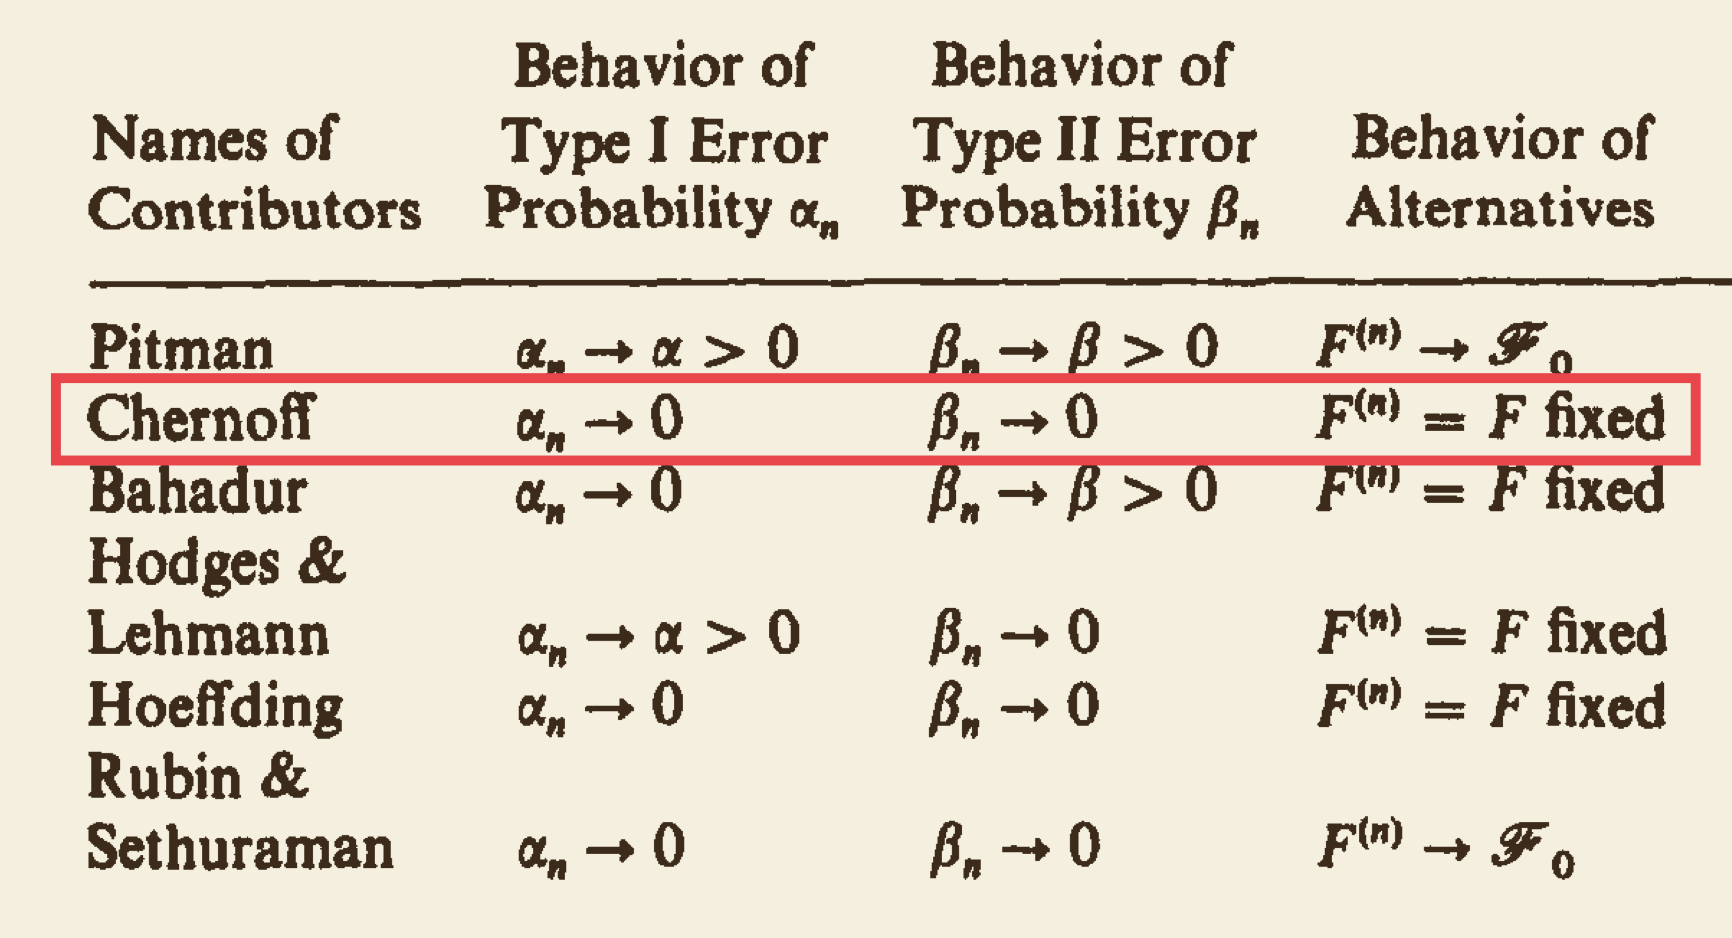
\includegraphics[width=0.9\textwidth]{figures/serflingAREtable.png}
  \end{figure}
  \hfill\link{end}{\huge back}

  \note{%

  }
\end{frame}


\bibliography{../library.bib}

\end{document}

